\documentclass{article}
\usepackage[utf8]{inputenc}
\usepackage{textcomp}
\usepackage[legalpaper, portrait, margin=1in]{geometry}
\usepackage{indentfirst}
\usepackage{graphicx}
\usepackage{amsmath}
\usepackage{amsfonts}
\usepackage{amssymb}
\usepackage{subfig}



\title{\textbf{The Logistic Equation With Delay}}
\author{\LARGE Connor Adams }
\date{\today}

\begin{document}


\maketitle

\setlength\parindent{0pt}

\textbf{\Large Abstract}
\bigskip

\setlength\parindent{10pt}

\indent \indent \large In this paper, I consider adding a lag element to the continuous logistic equation below:
   $$ \frac{dN}{dt} = rN(1-\frac{N}{k})\indent\indent (1),$$
Where $N(t)$ is the population at time $t$, $r$ is the growth rate, and $k$ is the carrying capacity of the population. Now that we have this logistic equation, we can alter it a little to help represent organisms who have some lag before they can reproduce. One way to take into account the lag is by using Delayed Differential Equations. So, the equation below is the recreation of equation (1):
$$ \frac{dN}{dt} = rN(1-\frac{N(t-\tau)}{k})\indent\indent (2),$$ Notice that we now have $N(t-\tau)$, where $\tau$ is the time delay that helps us create the lag. I then constructed a dimensionless form of equation (2): 
$$ \frac{dy}{dx} = \lambda y(1-y(x-1))\indent\indent (3),$$ 
This allowed me to observe our solutions using MATLAB and create plots which introduce that when $\lambda >\LARGE \frac{\pi}{2}$ the solution to the delayed-logistic equation starts an unstable oscillation. If $\lambda < \LARGE \frac{\pi}{2}$ then the solution will have a stable oscillation that tend toward $y = 1$. So, when $0 < \lambda < \LARGE \frac{\pi}{2}$ then equation (2) is stable and when $\lambda < \LARGE \frac{\pi}{2}$ then equation (2) is unstable. ultimately what we care about is the population $N(t)$ which we conclude that the equilibrium of said population is the carry capacity $N = k$. Lastly, when $r \tau > \frac{\pi}{2}$ $N = k$ is unstable and when
$r \tau < \frac{\pi}{2}$ $N = k$ is stable.
\bigskip
\hrule\hrule
\medskip

\section{Introduction}
\indent \indent Consider a continuous logistic equation that presumes the rate of change of the population changes
instantaneously to changes in the population like the one below:
$$\frac{dN}{dt} = rN(1-\frac{N}{k})\indent\indent (1),$$
where $N(t)$ is the population, $t$ is time, $r$ is the growth rate, and $k$ is the carry capacity It is more common to see organisms that have pulses of reproduction. Which means they have some lag before they are able to reproduce again. For example, looking at mammals that can pause their pregnancies until it is safe to resume again. Think of bears when they hibernate until spring arrives. This can be seen as a lag in their reproduction stage. So, introducing delay into the the logistic equation can help model these lags in reproduction. When introducing delay into equation (1) we get:
$$ \frac{dN}{dt} = rN(1-\frac{N(t-\tau)}{k})\indent\indent (2),$$
where $\tau$ will represent the lag. 

\bigskip
\hrule\hrule
\medskip

\section{Discussion of The Results and Project}

\subsection{Dimensionless Form}

\indent \indent First I start by deriving a dimensionless form of (2) where $y(x) = \frac{N(t)}{k}$ and $x = \frac{t}{\tau}$. So, equation (2) becomes:

$$\frac{\tau}{k} * \frac{dN}{dt} = \frac{\tau}{k} *  rN(1-\frac{N(t-\tau)}{k})$$
With some fun algebraic moves I get:
$$\frac{dN}{k} * \frac{\tau}{dt} = r\tau * \frac{N}{k} (1-\frac{N(t-\tau)}{k})$$
$$\frac{d(\frac{N}{k})}{d(\frac{t}{\tau})} = r\tau * \frac{N}{k} (1-\frac{N(t-\tau)}{k})$$
Using $y(x) = \frac{N(t)}{k}$ and $x = \frac{t}{\tau}$ I can simplify the equation to get:
$$\frac{dy}{dx} = r\tau y(1-\frac{N(t-\tau)}{k})$$
So, to evaluate $N(t-\tau)$ let $u =  x-1.$ and use $y(x) = \frac{N(t)}{k}$ and $x = \frac{t}{\tau}$ to show that because:
$$N(t) = N(\tau x) = k*y(x)$$
The results conclude that:
$$N(t-\tau) = N(\tau(x-1)) = N(\tau u) = k*y(u) = k*y(x-1)$$
So, input this back into the simplified equation and let $\lambda = r\tau$ to get:
$$\frac{dy}{dx} = \lambda y(1-\frac{k*y(x-1)}{k})$$
Lastly, the $k$ on the top cancels out the $k$ on the bottom which produces the final equation:
$$\frac{dy}{dx} = \lambda y(1-y(x-1) \indent\indent (3)$$ 
\subsection{Solutions}
\indent \indent Now that the logistic equation is in a dimensionless form, the solutions can be plotted when $\lambda = 1$ and $\lambda = 1.8$ with initial conditions $y = 0.5$ for $-1 < x < 0$ as presented below.

\bigskip
\begin{center}
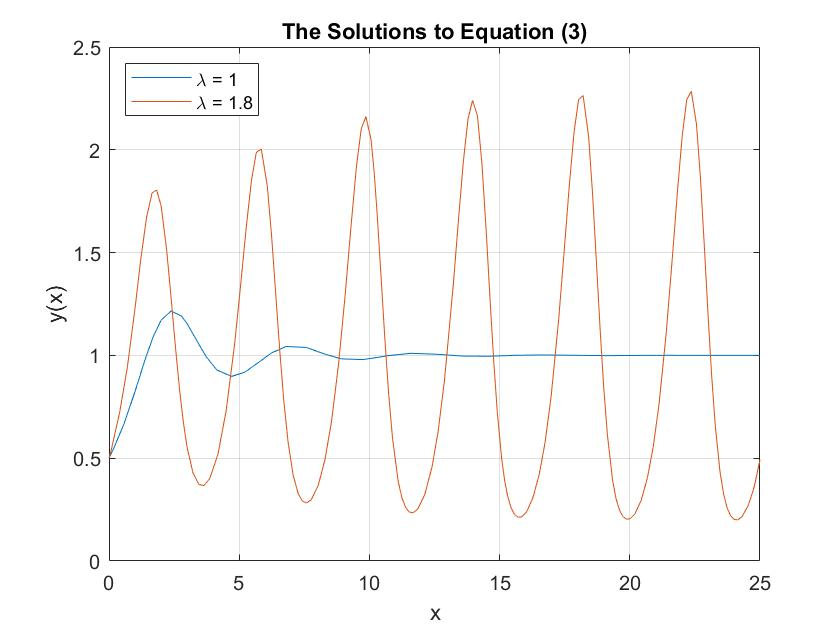
\includegraphics[width=15cm]{Solutions.jpg}

\textit{Figure 1: Solutions to equation (3) when $\lambda = 1$ and $\lambda = 1.8$}

\end{center}
\bigskip
Figure 1 is illustrating that $y(x)$ is a damped oscillation that converges to 1 when $\lambda = 1$ and $y(x)$ becomes a sustained oscillation when $\lambda = 1.8$. This implies that the solution $y(x) = 1$ is an equilibrium solution. The next question I asked myself is, at what value do the parameter $\lambda$ have to be at to produce the moment when the plot switches from converging to $0$ to maintaining a sustained oscillation? To do this we have to look at the stability of this delay-logistic equation.

\subsection{Stability}
\indent \indent Now that we know that the delay-logistic equation has an equilibrium at $y=1$, the stability at that equilibrium is under interrogation. By letting $u = y - 1$, the solutions to the  delay-logistic equation should be just shifted down by one, as well as the equilibrium. Substituting $u$ into equation (3) will help check to see if this bold statement is correct.
\newline Since, $$u = y-1$$
Then, $$y =  u+1$$
So, $$y(x-1) = u(x-1)+1$$
Therefore equation (3) becomes, $$\frac{du}{dx} = \lambda (u+1) (1-(u(x-1)+1)$$
After doing some simplification the result is revealed:
$$\frac{du}{dx} = -\lambda (u+1) (u(x-1))\indent\indent (4) $$
Below is the solutions to equation (4) when $\lambda = 1$ and when $\lambda = 1.8$:

\bigskip
\begin{center}
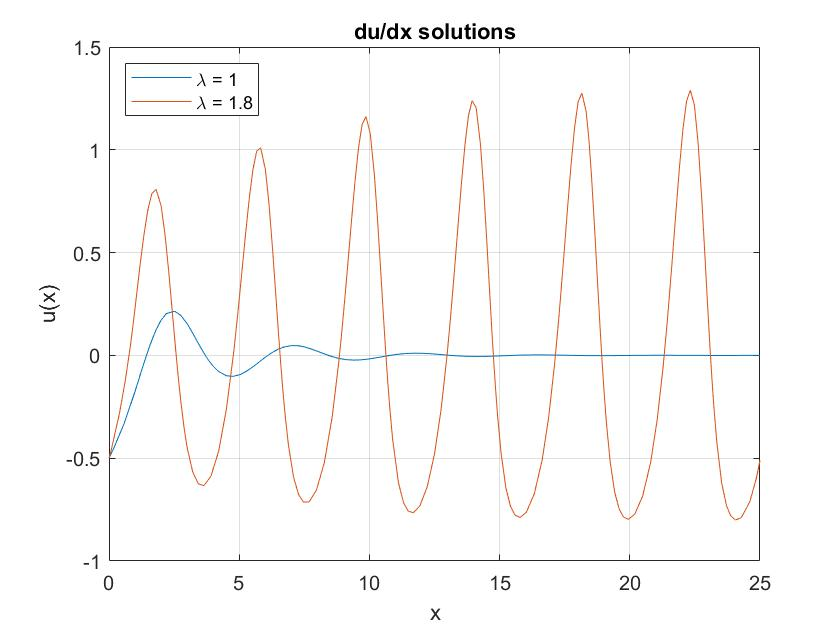
\includegraphics[width=15cm]{du solution 2 lam.jpg}

\textit{Figure 2: Solutions to equation (4) when $\lambda = 1$ and $\lambda = 1.8$}

\end{center}
\bigskip
This figure looks almost identical to figure 1, but the plot is just shifted down which confirms my earlier claim. The funny part is that this still doesn't represent the stability of the delay-logistic equation, but the equilibrium is at $y=1$, so when evaluating the stability at the equilibrium of $y=1$, but now $u=0$, equation (4) becomes:
$$\frac{du}{dx} = -\lambda u(x-1)\indent\indent (5)$$
Now, suppose that (5) has a solution of the form $u(x) = e^{hx}$. Then, with a little elbow grease we get:
$$he^{hx} = -\lambda e^{h(x-1)} = -\lambda e^{hx} e^{-h}$$
Divide both sides by $e^{hx}$:
$$h = -\lambda e^{-h}$$
Separate variables:
$$-he^h = \lambda$$
Let $h = w +iv$:
$$-(w+iv)e^{w+iv} = \lambda$$
Do algebraic sorcery:
 $$(-w-iv) e^w e^{iv} = \lambda$$
Move $e^w$ to the other side:
$$(-w-iv) e^{iv} = \lambda e^{-w}$$
Now for some complex analysis sorcery:
$$(-w-iv) (\cos{(v)} + i\sin{(v)}) = \lambda e^{-w}$$
More algebraic sorcery:
$$ -w\cos{(v)} + v\sin{(v)}) - i(v\cos{(v)} + w\sin{(v)}) = \lambda e^{-w} \indent \indent (6)$$
With this, we can separate (6) into real and imaginary parts:

\begin{center}
\underline{REAL PART:}
$$\boxed{\lambda = (-w\cos{(v)} + v\sin{(v)}) e^w}$$
\underline{IMAGINARY PART:}
$$\boxed{0 = -(v\cos{(v)} + w\sin{(v)})}$$
\end{center}
By evaluating the real part we can see that if $w > 0$ the solutions for (5) will oscillate with growing amplitude because 
$(-w\cos{(v)} + v\sin{(v)})$ will create the oscillation and $e^w$ will create the growing amplitude. The imaginary part will be $0$, 
so there is no need to look at that part. Also, If $w < 0$ the solutions will converge toward $0$. The more interesting part is if $w = 0$ what happens to the the solutions:

\begin{center}
    \underline{If $w = 0$}
\end{center}
Then, the real and imaginary parts become:
\begin{center}
\underline{REAL PART:}
$$\boxed{\lambda = v\sin{(v)}}$$
\underline{IMAGINARY PART:}
$$\boxed{0 = -v\cos{(v)}}$$
\end{center}
Now, $cos(v) = 0$ when $v = \frac{2k+1}{2}\pi$, where $k \in \mathcal{Z}$. This implies that $\sin{(v)} = 1$ when 
$v = \frac{\pi}{2} + 2k\pi$, and $\sin{(v)} = -1$ when $v = \frac{-\pi}{2} + 2k\pi$ where $k \in \mathcal{Z}$. 
$$\boxed{\therefore \indent \indent \lambda = \frac{2k+1}{2}\pi, \indent \indent k \in \mathcal{Z}}$$
So, to make things simple for our plot if $ w = 0 $ then $\lambda = \frac{\pi}{2}$ and the solutions for (5) will have a sustained oscillation. Also, if $ w > 0 $ then $\lambda > \frac{\pi}{2}$ and if $ w < 0 $ then $\lambda < \frac{\pi}{2}$ which will prove useful when looking at the figure below.

\bigskip
\begin{center}
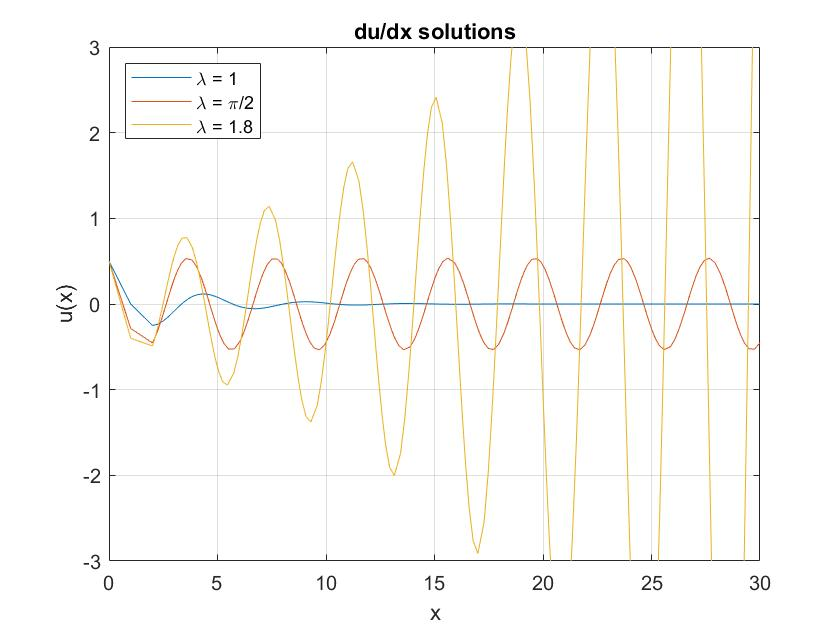
\includegraphics[width=15cm]{du solutions.jpg}

\textit{Figure 3: Solutions to equation (5) when $\lambda = 1$, $\lambda = \frac{\pi}{2}$, and $\lambda = 1.8$}

\end{center}
Figure 3 represents all 3 cases. Notice that when $\lambda = 1$ the solution tends toward $0$, when $\lambda = 1.8$ the solution oscillates with a growing amplitude, and finally when $\lambda = \frac{\pi}{2}$ the solution oscillates with a stable amplitude. In my opinion plotting equation (5) gives a better picture than the other equations when looking close the parameter, $\lambda = \frac{\pi}{2}$, for the delay-logistic equation. For example:

\bigskip
\begin{center}
    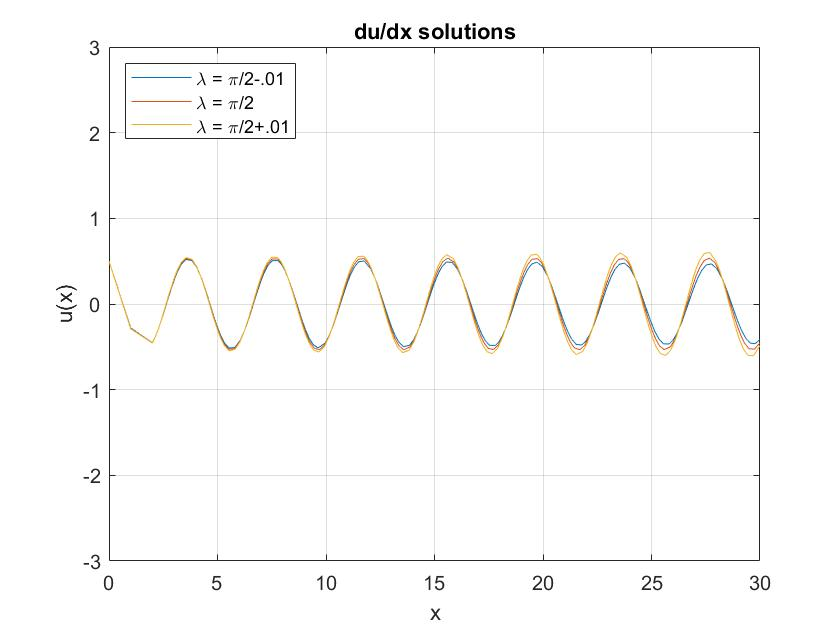
\includegraphics[width=9.5cm]{du_close1.jpg}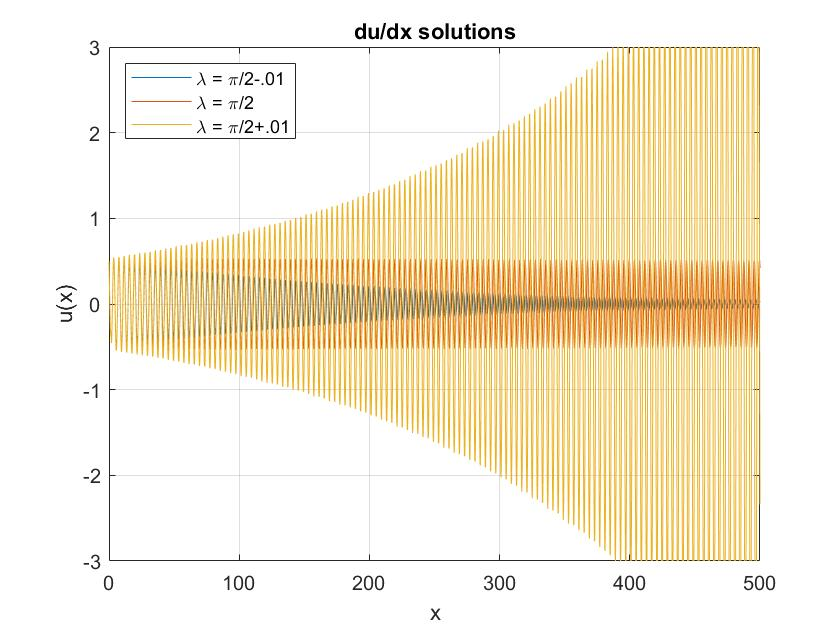
\includegraphics[width=9.5cm]{du_close2.jpg}
    
    \textit{Figure 4: Solutions to equation (5) when $\lambda = \frac{\pi}{2}-.01$, $\lambda = \frac{\pi}{2}$, and $\lambda = \frac{\pi}{2}+.01$}
    
\end{center}
In Figure 4 there are two of the same plots, just over a different time period. In the first graph, notice how the 3 curves look almost identical and it is hard to see the difference. Now in the second graph, with a large enough time frame all 3 curves look drastically different. the amplitude of the yellow curve is growing toward infinity, the orange curve is oscillating at a constant amplitude, and the blue curve has an amplitude that is converging to $0$. These 2 plots are a great representation of what happens when the parameter $\lambda$ is around $\frac{\pi}{2}$. So to conclude, if $\lambda > \frac{\pi}{2}$ then $y=1$ is unstable and if $\lambda < \frac{\pi}{2}$ then $y=1$ is stable. 


\bigskip
\hrule\hrule
\medskip

\section{References}

\begin{thebibliography}{}
\bibitem{ScienceDirect}
Juan Cui: Delay differential logistic equation with linear harvesting,
\\\texttt{https://www.sciencedirect.com/science/article/abs/pii/S1468121806001040}

\bibitem{Rand}
Richard Bellman and Kenneth L. Cooke: Delayed-Differential Equations,
\\\texttt{https://www.rand.org/content/dam/rand/pubs/reports/2006/R374.pdf}

\bibitem{Arxiv}
Dongcai: Stability analysis of delay differential equations via Semidefinite programming,
\\\texttt{https://arxiv.org/ftp/arxiv/papers/1610/1610.07308.pdf}

\bibitem{math.fsu}
Bertram: Delay-Differential Equations,
\\\texttt{https://www.math.fsu.edu/~bertram/lectures/delay.pdf}

\bibitem{cs.kuleuven}
EngelBoghs: DDE-BIFTOOL: a Matlab package for bifurcation analysis of delay differential equations,
\\\texttt{http://www.cs.kuleuven.be/publicaties/rapporten/tw/TW305.pdf}

\bibitem{math.le}
Davidchack: Lab 3: Bifurcation diagrams,
\\\texttt{http://www.math.le.ac.uk/people/rld8/ma1251/lab3.html}

\bibitem{Sciencealert}
Fenelon: Some Animals Can Literally Pause Their Pregnancies. Here's Why,
\\\texttt{https://www.sciencealert.com/some-animals-can-literally-pause-their-pregnancies-here-s-why}

\bibitem{Ruan-nato}
Ruan: DELAY DIFFERENTIAL EQUATIONS IN SINGLE SPECIES DYNAMICS,
\\\texttt{https://www.math.miami.edu/~ruan/MyPapers/Ruan-nato.pdf}

\bibitem{DDE-Chapter3}
Rand: Chapter 3 Differential-Delay Equations,
\\\texttt{http://pi.math.cornell.edu/~rand/randpdf/DDE-chapter3.pdf}

\bibitem{LimitCyclesandChaos}
Sharov: 9.5. Limit Cycles and Chaos,
\\\texttt{http://pi.math.cornell.edu/~rand/randpdf/DDE-chapter3.pdf}

\bibitem{paper}
Wright and Fox: Delay Differential Equations and the Logistic Population Model,
\\\texttt{https://mse.redwoods.edu/darnold/math55/DEproj/sp12/wright/paper.pdf}

\bibitem{09_delay_oscillators}
Bois and Elowitz: 9. Delay oscillators,
\\\texttt{http://be150.caltech.edu/2019/handouts/09_delay_oscillators.html}

\end{thebibliography}

\bigskip
\hrule\hrule
\medskip

\section{Source code}

\begin{center}
    \LARGE Figure 1 code:
    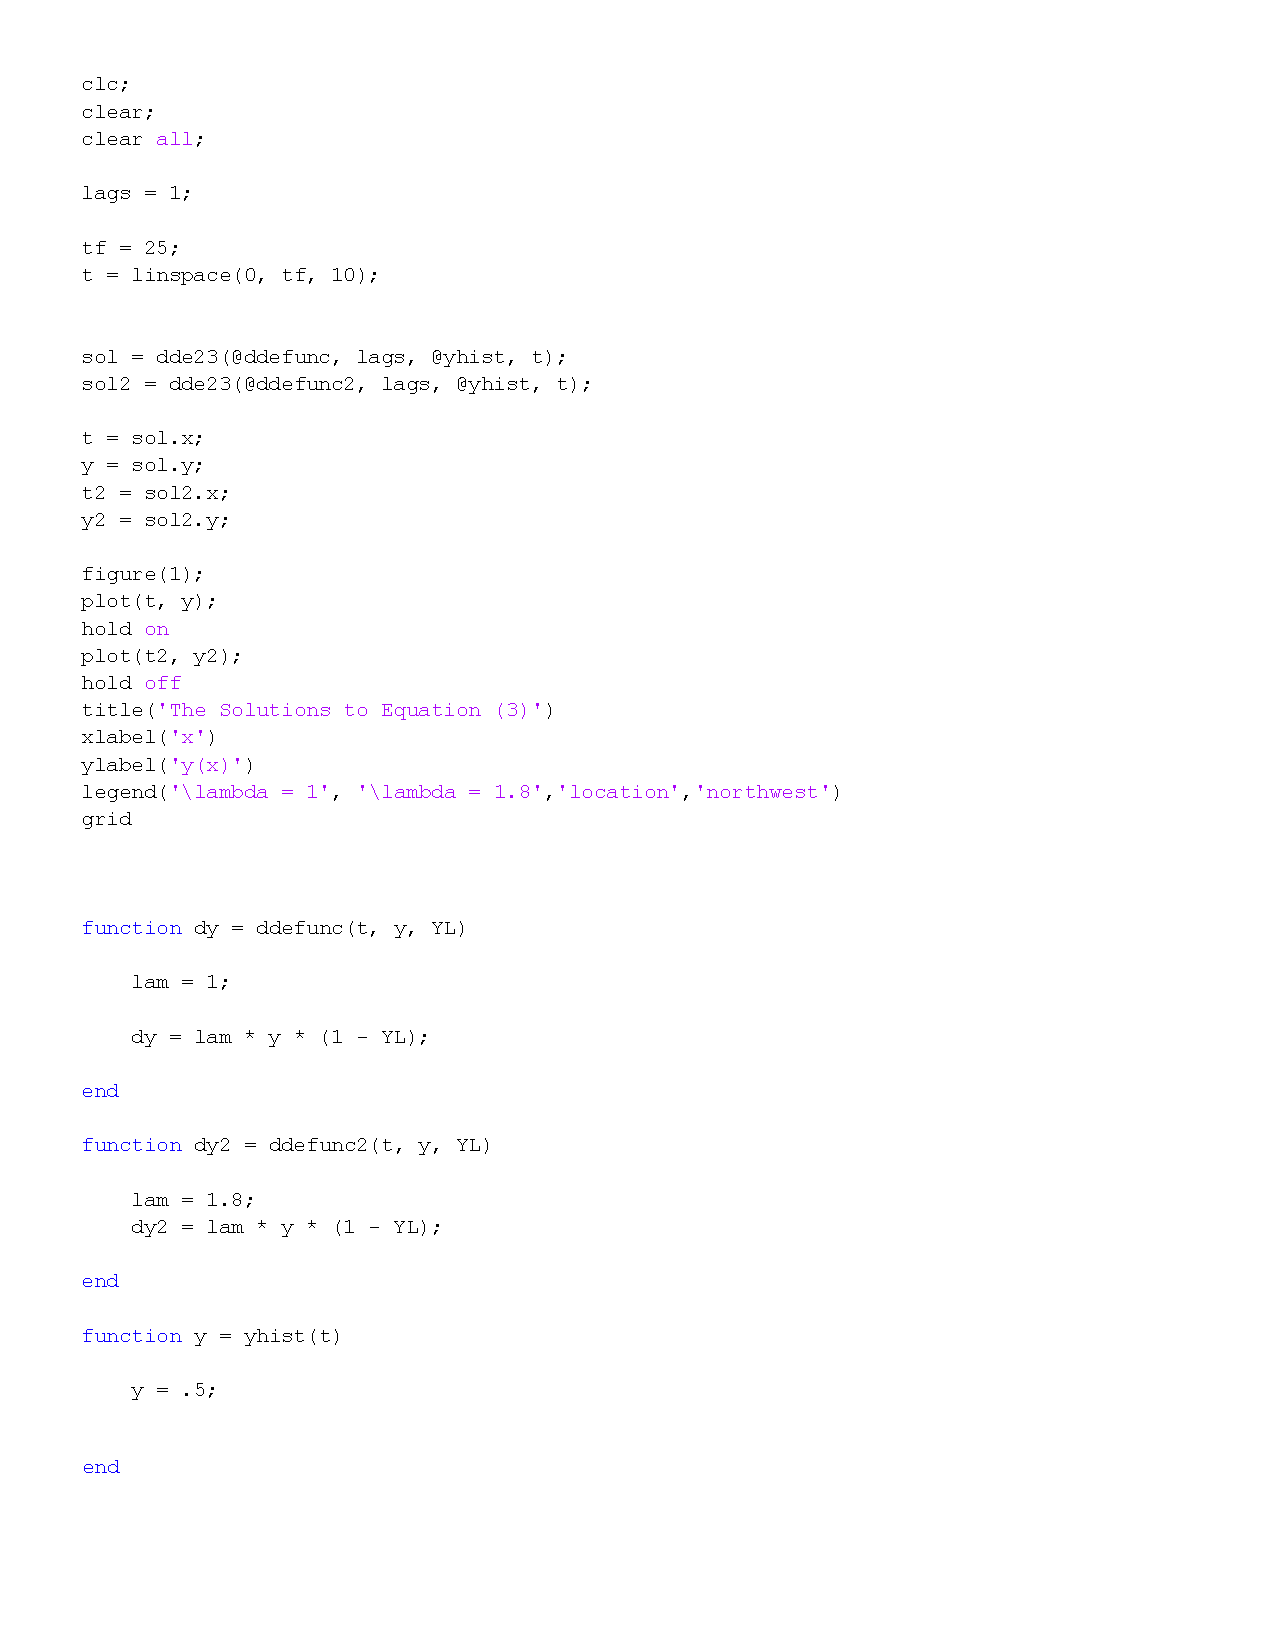
\includegraphics[width=15cm]{Figure_1.pdf}
\end{center}
\newpage
\begin{center}
    \LARGE Figure 2 code:
    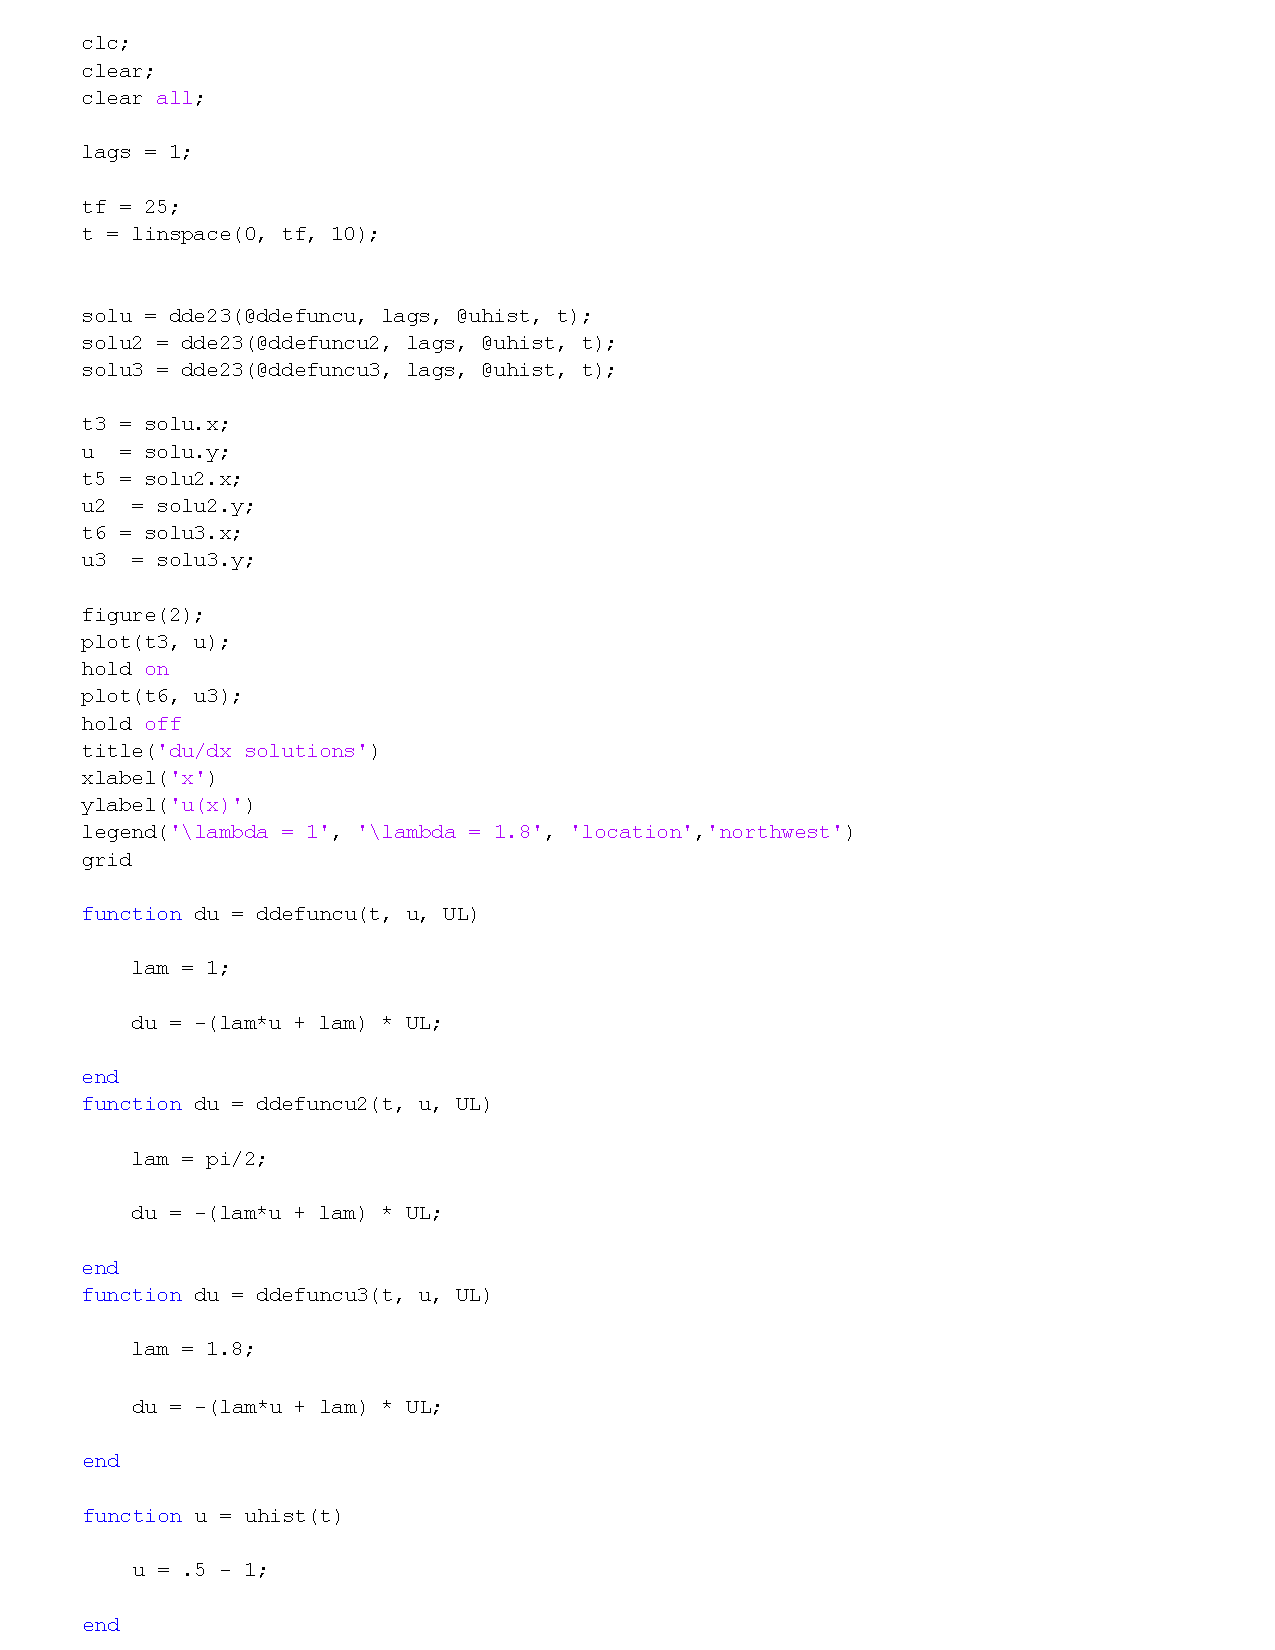
\includegraphics[width=15cm]{Figure_2I.pdf}
\end{center}
\newpage
\begin{center}
    \LARGE Figure 3 code: 
    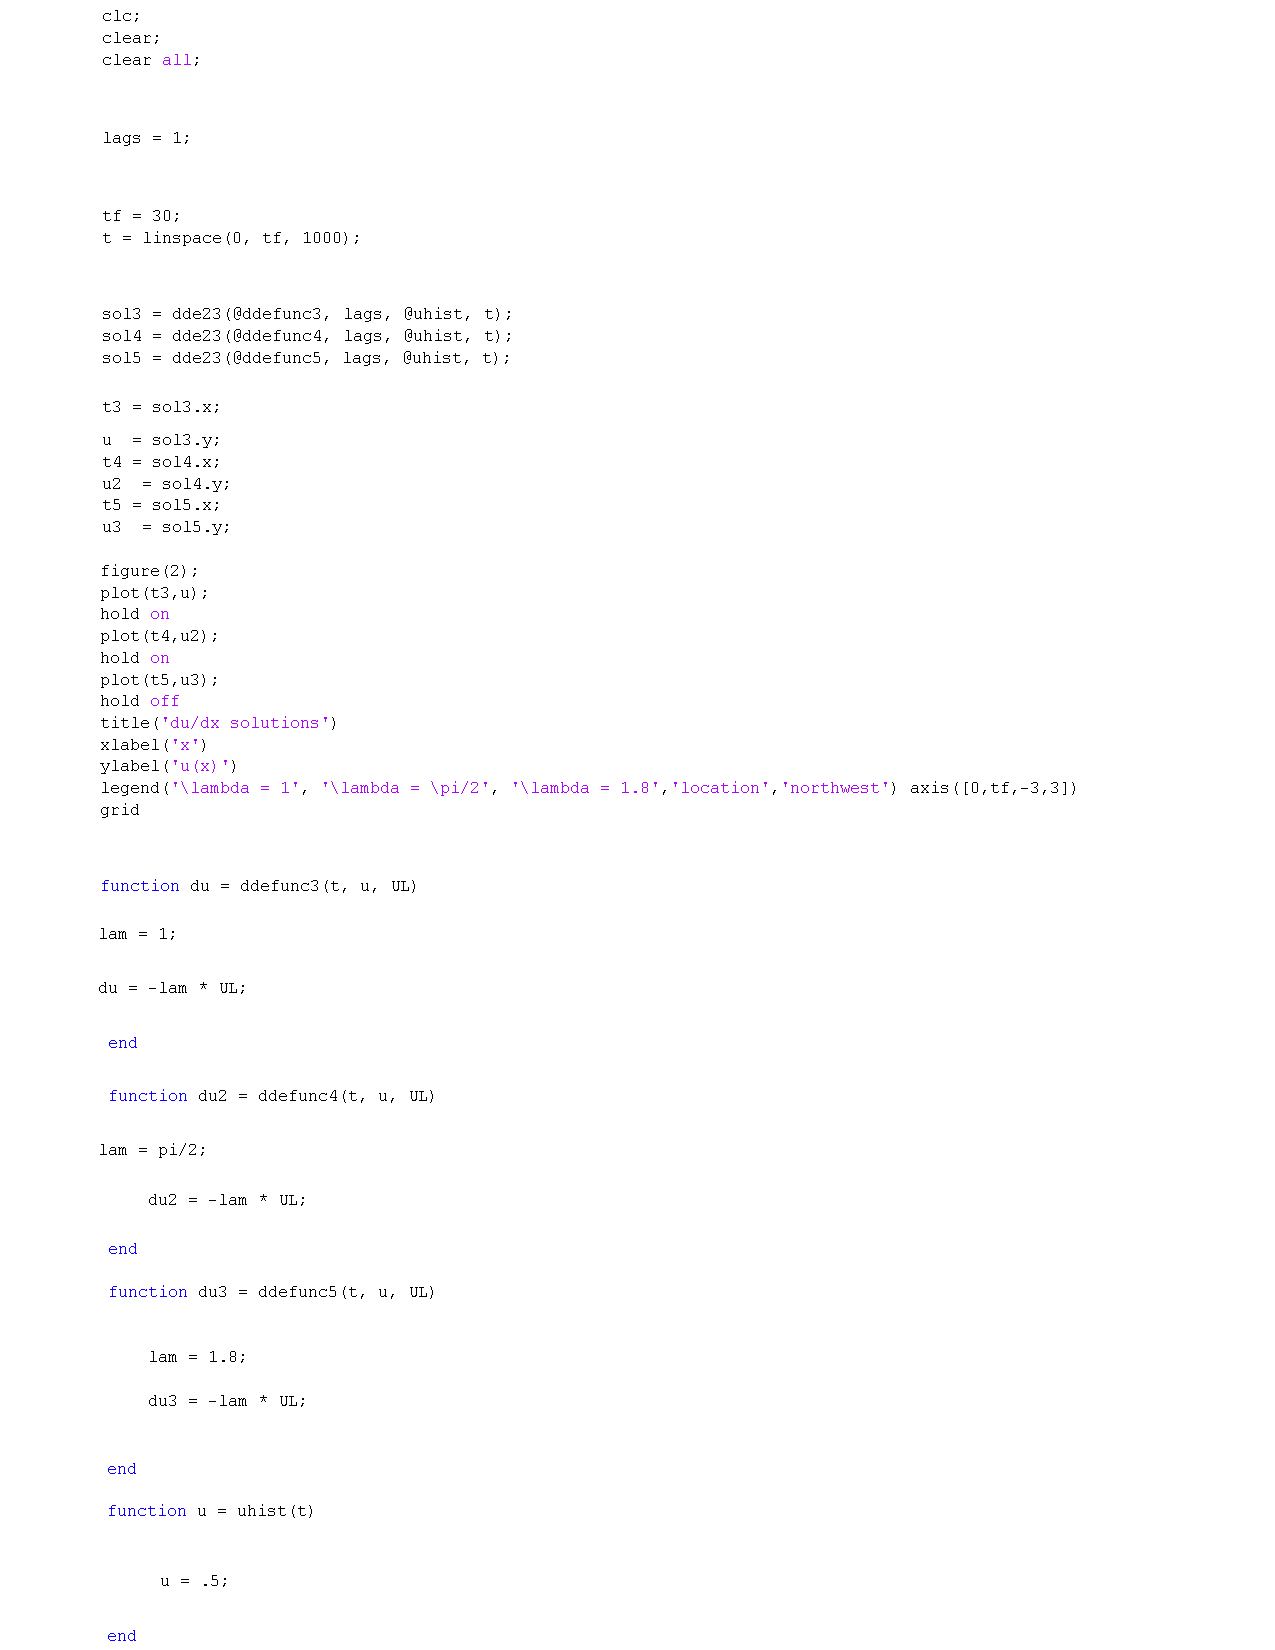
\includegraphics[width=15cm]{du_solutions(5).pdf}
\end{center}
\newpage
\begin{center}
    \LARGE Figure 4 code: 
    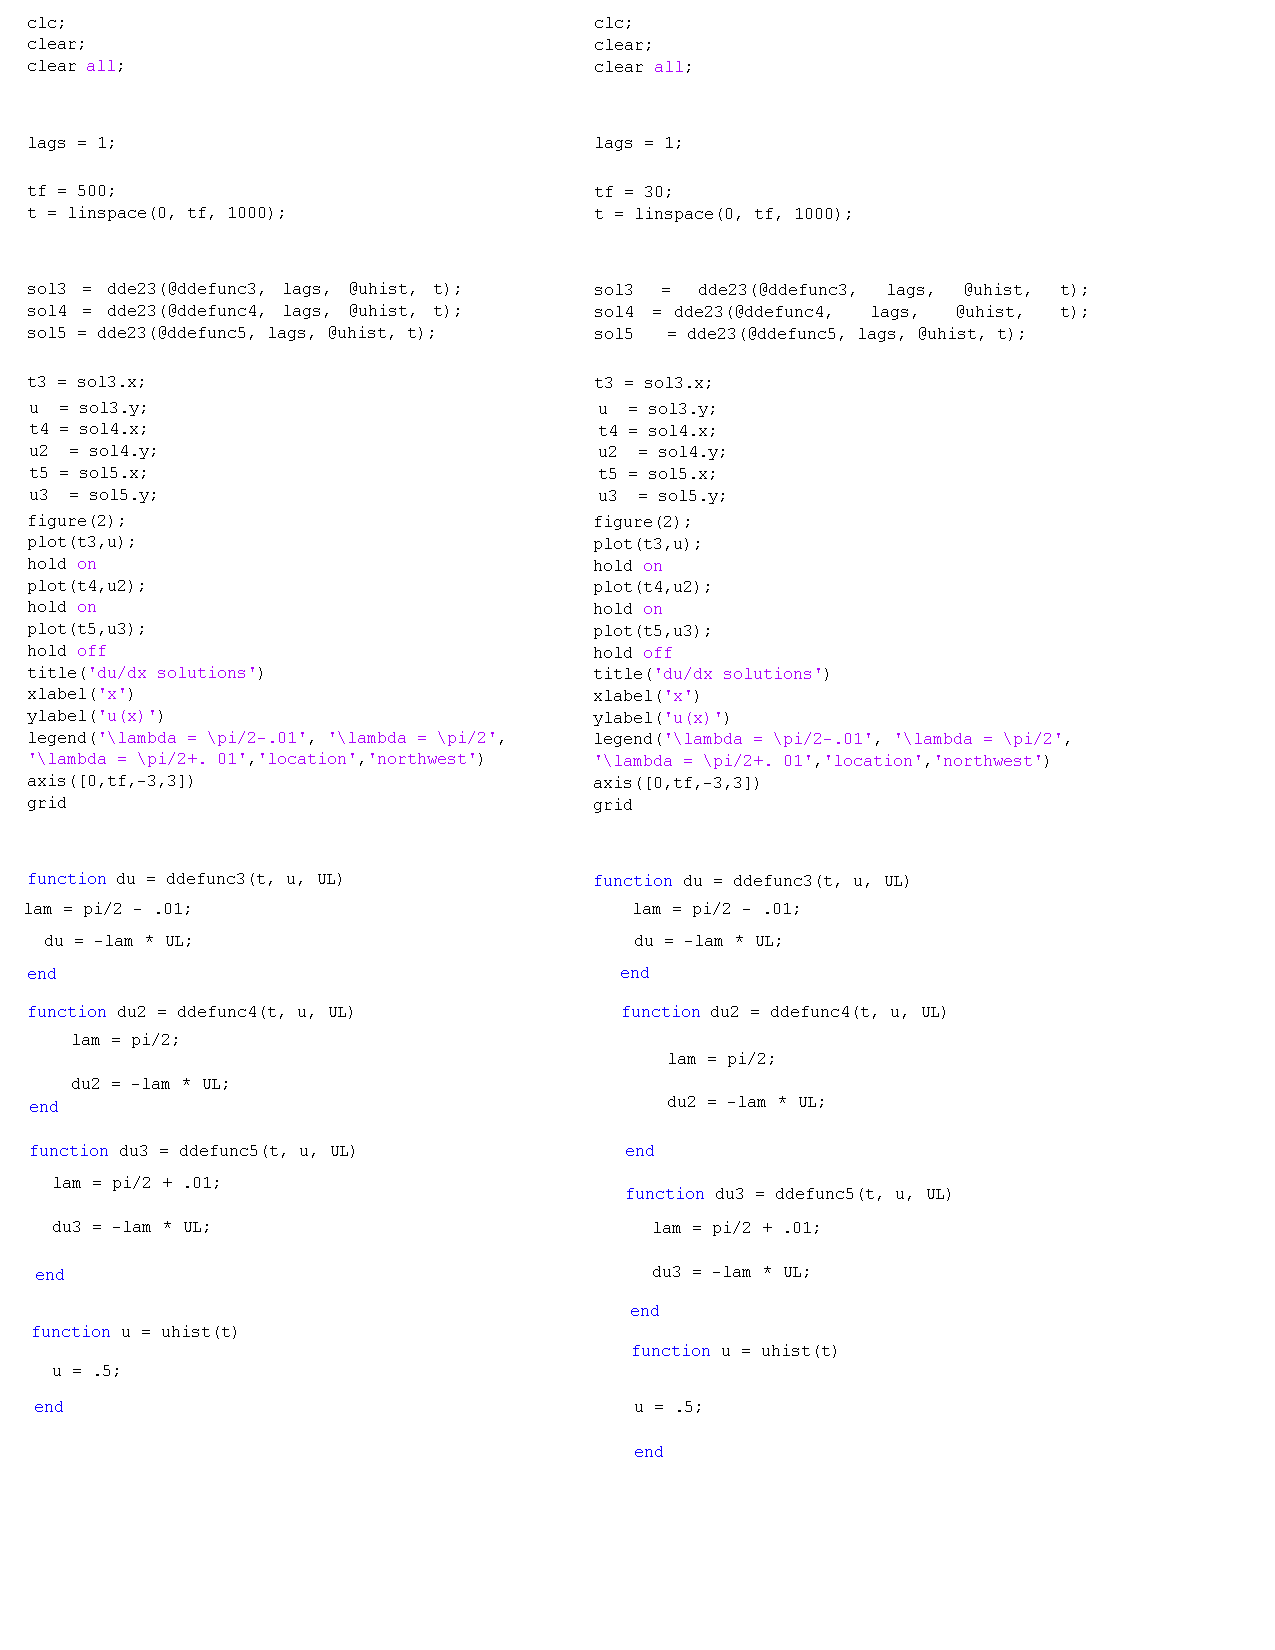
\includegraphics[width=15cm]{lam_close.pdf}
\end{center}

\end{document}
